\documentclass{standalone}

\usepackage{pgfplots}
\usepackage{amssymb}
\usepackage{amsmath}

\DeclareMathOperator*{\wt}{wt}

\pgfplotsset{compat=1.17}

\begin{document}

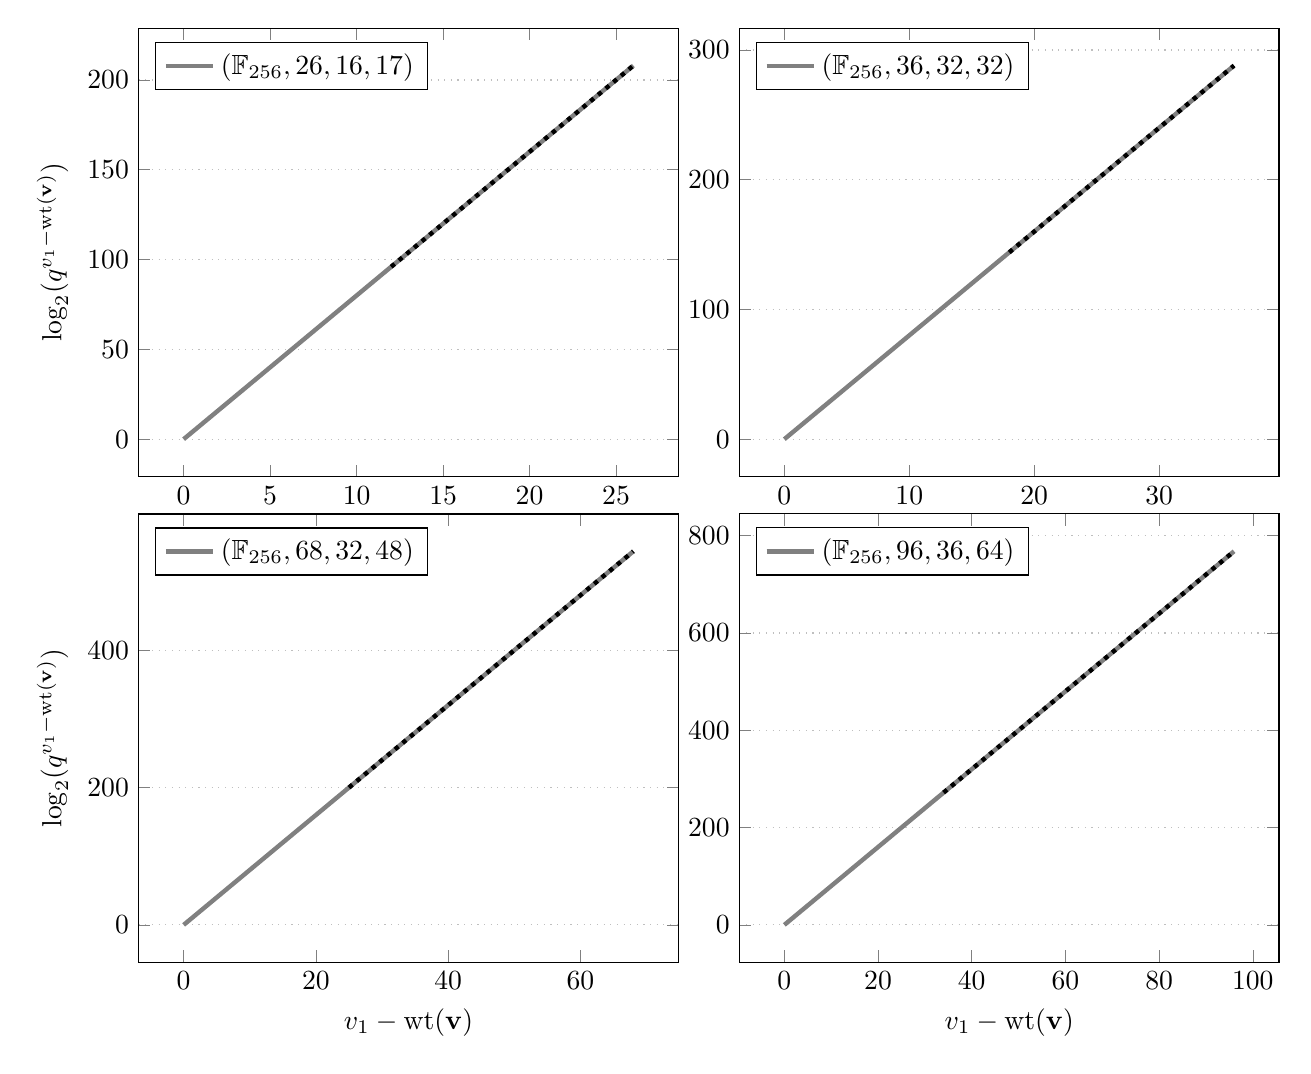
\begin{tikzpicture}
  \begin{axis}[
    name = plot1,
    legend pos = north west,
    ylabel = $\log_{2}(q^{v_{1} - \wt(\mathbf{v})})$,
    ymajorgrids = true,
    grid style = dotted,
  ]
    \addplot[gray, ultra thick, domain=0:26] { log2(256^(x)) };
    \addplot[black, dotted, ultra thick, domain=12:26] { log2(256^(x)) };
    \addlegendentry{$(\mathbb{F}_{256}, 26, 16, 17)$};
  \end{axis}

  \begin{axis}[
    name = plot2,
    at = (plot1.right of south east),
    anchor = left of south west,
    legend pos = north west,
    ymajorgrids = true,
    grid style = dotted,
  ]
    \addplot[gray, ultra thick, domain=0:36] { log2(256^(x)) };
    \addplot[black, dotted, ultra thick, domain=18:36] { log2(256^(x)) };
    \addlegendentry{$(\mathbb{F}_{256}, 36, 32, 32)$};
  \end{axis}

  \begin{axis}[
    name = plot4,
    at = (plot2.below south west),
    anchor = above north west,
    legend pos = north west,
    xlabel = $v_{1} - \wt(\mathbf{v})$,
    ymajorgrids = true,
    grid style = dotted,
  ]
    \addplot[gray, ultra thick, domain=0:96] { log2(256^(x)) };
    \addplot[black, dotted, ultra thick, domain=34:96] { log2(256^(x)) };
    \addlegendentry{$(\mathbb{F}_{256}, 96, 36, 64)$};
  \end{axis}

  \begin{axis}[
    name = plot3,
    at = (plot4.left of south west),
    anchor = right of south east,
    legend pos = north west,
    xlabel = $v_{1} - \wt(\mathbf{v})$,
    ylabel = $\log_{2}(q^{v_{1} - \wt(\mathbf{v})})$,
    ymajorgrids = true,
    grid style = dotted,
  ]
    \addplot[gray, ultra thick, domain=0:68] { log2(256^(x)) };
    \addplot[black, dotted, ultra thick, domain=25:68] { log2(256^(x)) };
    \addlegendentry{$(\mathbb{F}_{256}, 68, 32, 48)$};
  \end{axis}
\end{tikzpicture}

\end{document}
